%!TEX root = skripsi.tex
%-----------------------------------------------------------------------------%
\chapter{\babEmpat} \label{implementasi}
%-----------------------------------------------------------------------------%
Bab ini akan menjelaskan perihal implementasi dari pemindahan \textit{sense} dan sistem \textit{WSD} yang dibuat.


\section{\textit{Word Alignment}}

\subsection{Pre-Processing}
Perlu dilakukan \textit{pre-processing} untuk memisahkan kalimat bahasa Inggris dan bahasa Indonesia menjadi dua buah \textit{file} paralel untuk dapat dimasukan sebagai input dari \textit{tool} Giza.

\begin{figure}
	\centering
	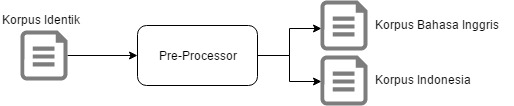
\includegraphics[width=1\linewidth]{adit_pics/pre-process-giza}
	\caption{Pre-Processing Giza}
	\label{fig:Pre-Processing-Giza}
\end{figure}

\subsection{Pemrosesan \textit{Word Alignment}}
Setelah kedua buah korpus bahasa Indonesia dan Inggris terpisah, perintah berikut digunakan untuk melakukan \textit{alignment} dengan Giza pada penelitian ini:

\begin{lstlisting}[language=bash,caption={Word Alignment}, label={word-alignment}]
# Lakukan pada direktori Giza
./plain2snt.out [source_language] [target_language]

# proses diatas menghasilkan tiga buah file yaitu dua buah file vocabulary yang berisi indeks dengan kata (bahasa asal, dan bahasa tujuan), dan satu buah file snt yang berisi \textit{alignment} dari kalimat.

./snt2cooc.out [source_language_vcb_file] [target_language_vcb_file] [snt_file] > [coocurrence_file]

# proses snt2cooc akan menghasilkan \textit{cooccurence file}

./GIZA++ -S [source_language_vcb] -T [target_language_vcb] -C [snt_file] -CoocurrenceFile [cooc_file]
\end{lstlisting}

Giza mengeluarkan beberapa \textit{file} hasil dari proses tersebut. \textit{Output} yang akan digunakan diantaranya adalah \textit{file} bernama A3.final yang merupakan pasangan kalimat dengan kata-kata yang sudah dipasangkan sesuai dengan prediksi terbaik hasil pemrosesan Giza.

\subsection{Post-Processing}
Setelah mendapatkan \textit{file} A3 dari Giza, dilakukan \textit{post-processing} untuk menghasilkan file yang dengan mudah dapat diproses untuk melakukan \textit{sense transfering}.

Berikut ini merupakan salah satu contoh pasangan kalimat pada \textit{file} A3 keluaran Giza:

\begin{lstlisting}caption={A3-File}, label={a3-file}]
# Sentence pair (47183) source length 9 target length 9 alignment score : 6.85298e-13
Undang-Undang No 14 tahun 2008 tentang Kebebasan Memperoleh Informasi 
NULL ({ }) Law ({ 1 }) No ({ 2 }) 14 ({ 3 }) of ({ }) 2008 ({ 4 5 }) on ({ 6 }) Freedom ({ 7 8 }) of ({ }) Information ({ 9 })
\end{lstlisting}

Pembacaan pasangan kata berdasarkan hasil keluaran dilakukan dengan indeks nomor kata yang berada pada dalam kurung kata di bahasa Inggris. Karena pemisah token \textit{by default} adalah spasi, maka kata "Undang-Undang" adalah kata dengan indeks nomor 1, kata "No" adalah kata dengan indeks nomor 2, dan berlaku hal yang sama sampai kata "Informasi". Pada kata bahasa inggris, "Law" dipasangkan dengan indeks satu yang mana adalah "Undang-Undang", kata "No" dipasangkan dengan indeks dua yang mana adalah "No". 

Terdapat dua buah \textit{post-processing} yang dilakukan dengan tujuan masing-masing untuk:

\begin{enumerate}
	\item Penyimpan pasangan kata-kata yang bersesuaian untuk sistem WSD.
	\item Sebagai \textit{resource} untuk proses \textit{enhancement word alignment}.
\end{enumerate}


Untuk keperluan nomor satu, bentuk \textit{output} diproses menjadi bentuk lain dengan format:

\begin{lstlisting}
<pair>kata_en_1||kata_id_1 kata_id_2</pair?##<pair>kata_en_2||kata_id\_3</pair>...</pair>
\end{lstlisting}

Contoh dari hasil \textit{post-processing} pada pasangan kalimat sebelumnya adalah:

\begin{lstlisting}
<pair>law||undang-undang</pair>##<pair>no||no</pair>##<pair>14||14</pair>##<pair>2008||tahun 2008</pair>##<pair>on||tentang</pair>##<pair>freedom||kebebasan memperoleh</pair>##<pair>information||informasi</pair>
\end{lstlisting}

Hasil ini kemudian disimpan sebagai sebuah \textit{file} sendiri yang akan digunakan kembali pada sistem WSD nantinya. Sementara itu, keperluan nomor dua difokuskan untuk membuat \textit{dictionary} yang akan ditingkatkan kualitasnya pada tahap berikutnya. Untuk menghasilkan \textit{file} yang dibutuhkan pada nomor kedua, dilakukan pengumpulan pasangan kata bahasa Indonesia dengan bahasa Inggris. Bila misalkan pada kalimat ke-n terdapat kata "undang-undang" yang dipasangkan dengan "law", dan pasangan kata "undang-undang" dengan "regulation" pada kalimat lain (kalimat ke-m, dimana m != n). Berdasarkan kedua kalimat tersebut, maka kata "undang-undang" akan berpasangan dengan dua kata yaitu "law", dan "regulation".

\section{Peningkatan Kualitas \textit{Alignment}}

Hasil dari \textit{alignment} kata yang dilakukan Giza masih menghasilkan pasangan-pasangan kata yang tidak tepat. Untuk mengurangi jumlah pasangan kata yang salah tersebut, dilakukan \textit{enhancement} dengan dua kali proses \textit{alignment} baik itu dari Indonesia ke Inggris maupun sebaliknya.

Konsep dari proses yang dilakukan adalah melakukan validasi terhadap kata-kata yang berpasangan  dari kedua korpus. Pertama, setiap kata dalam bahasa Indonesia dikumpulkan terlebih dahulu dengan setiap pasangan kata bahasa Inggrisnya (satu kata bisa memiliki lebih dari satu pasangan). Proses selanjutnya adalah melakukan pengumpulan yang serupa terhadap kata dalam bahasa Inggris dengan pasangan kata dalam bahasa Indonesianya. Proses validasi dilakukan dengan cara:

\begin{enumerate}
	\item Untuk setiap kata di bahasa Indonesia semisal kata "kali"
	\item Lakukan pengecekan terhadap setiap pasangan kata di bahasa Inggris dari "kali" misalkan "time", "river", "fire"
	\item Jika pada kamus \textit{enhancement} "time" dipasangkan dengan "kali", dan "waktu" maka kata "time" merupakan pasangan yang dianggap benar. Pada kasus kata "fire", bila pasangan bahasa Indonesianya adalah "api" dan "tungku", maka kata "fire" dianggap bukan pasangan yang tepat dengan "kali" karena tidak terdapat pasangan "fire -> kali".
\end{enumerate} 

\begin{lstlisting}[language=Python, caption={Word Alignment Enhancement}, label={word-alignment-enhancement}]

dict_id = {}
dict_en = {}

# masukan setiap kosa kata bahasa Indonesia ke dalam dict_id sebagai key dan kumpulan pasangan kata bahasa inggrisnya sebagai value
# proses yang sama dilakukan untuk dict_en dengan kosa kata bahasa Inggris sebagai key dan kumpulan pasangan kata bahasa Indonesia sebagai value
# stop adalah list stopword yang didapat dari korpus nltk

# this section is for filtering which english word that has corresponding indo translation (bidirectional) from Giza output
for indo_word in dict_id.keys():
if indo_word not in dict_en:
# filtering so no same translation is entered, answer -> answer, jawaban -> jawaban
for en_word in dict_id[indo_word].keys():
if en_word in dict_en and indo_word in dict_en[en_word] and en_word not in stop:
if indo_word not in final_dictionary:
final_dictionary[indo_word] = { en_word: dict_en[word_en][word_id] }
else:
if en_word not in final_dictionary[indo_word]:
final_dictionary[indo_word][en_word] = dict_en[word_en][word_id]
\end{lstlisting}


\section{Pemindahan Makna Kata}
Hasil dari proses peningkatan kualitas \textit{alignment} adalah sebuah kamus bahasa yang akan digunakan sebagai referensi untuk memindahkan makna kata dari bahasa Inggris ke kata pada bahasa Indonesia.


%-----------------------------------------------------------------------------%
\section{Sistem WSD}
Sistem WSD dibangun dengan menggunakan \textit{supervised learning}. \textit{Machine learning tool} yang digunakan untuk membangun sistem ini adalah Scikit \citep{scikit-learn}. Pada sistem ini terdapat tiga buah bagian utama yaitu pemilihan fitur serta \textit{classifier}, ekstraksi fitur, dan evaluasi hasil \textit{classifier}.

\subsection{Pemilihan Fitur dan \textit{Classifier}}
Terdapat tiga buah fitur pada penelitian ini yang terdiri dari:

\begin{enumerate}
	\item Fitur \textit{bag of words}
	\item Fitur \textit{POS tagging}
	\item Vektor dari hasil \textit{word embedding}
\end{enumerate}

\textit{Classifier} yang digunakan pada penelitian ini adalah SVM dengan \textit{library} Python yaitu Scikit dengan parameter \textit{default} berupa kernel linear dan C=1.

\subsection{Ekstraksi Fitur}
Fitur bag of words menggunakan pendekatan kemunculan kata-kata pada konteks kalimat sebagai fitur. Kata yang diambil untuk dijadikan fitur adalah dua buah kata di kiri dan di kanan dari \textit{target word}. Pada penelitian ini, kata-kata yang merupakan bagian dari \textit{stopwords} dalam bahasa Indonesia tidak dimasukan sebagai fitur. Contoh dari fitur ini dapat dilihat pada kalimat dengan kata tujuan "bisa" berikut:
\\
- Ani digigit ular dengan bisa yang berbahaya
\\
Pada contoh kalimat tersebut, \textit{bag of words} yang diambil adalah ["digigit", "ular", "berbahaya", NULL]

Setiap fitur \textit{bag of words} dari setiap kalimat tersebut dikumpulkan untuk menjadi satu fitur besar yang mendeteksi kemunculan kata-kata tersebut pada setiap kalimat.

Proses yang dilakukan dalam pengambilan kata konteks untuk fitur \textit{bag of words} dilakukan dengan tahap-tahap berikut.

\begin{lstlisting}[language=python,caption={Fitur Bag of Words}, label={fitur-bag-of-words}]

bag_of_words []

for each sentence
	split sentence by whitespace into words
	for each word
		if word == target word
			for x in [-2,-1,1,2]
				if word(x) exist and word(x) not in bag_of_words
					add word(x) into bag_of_words
					
return bag_of_words

\end{lstlisting}

Fitur POS Tagging menggunakan \textit{tool} dari Stanford bernama "A Part-Of-Speech Tagger" yang dilatih dengan menggunakan model untuk bahasa Indonesia. Proses \textit{tagging} ini dilakukan sebelum memasuki sistem WSD terhadap keseluruhan kalimat dalam korpus identik yang berisi bahasa Indonesia saja. Terdapat \textit{pre-processing} awal pada korpus bahasa Indonesia tersebut untuk menghilangkan beberapa tanda baca seperti titik, koma, tanda tanya, tanda seru, dan beberapa tanda baca lainnya. Setelah proses tersebut, diberikan tanda baca berupa titik pada akhir kalimat sebagai indikator akhir sebagai kebutuhan dari kompabilitas \textit{tool} (tidak semua kalimat pada korpus memiliki tanda baca akhir kalimat). Perintah yang dilakukan untuk melakukan \textit{POS Tagging} tersebut adalah:

\begin{lstlisting}[language=bash,caption={Stanford POS Tagger}, label={stanford-pos-tagger}]

java -mx300m -cp 'stanford-postagger.jar:lib/*' edu.stanford.nlp.tagger.maxent.MaxentTagger -model <model_bahasa_indonesia> -textFile <korpus_bahasa_indonesia>

\end{lstlisting}

Hasil dari proses tersebut merupakan korpus dengan setiap kata yang sudah memiliki POS Tag dengan format:

\begin{lstlisting}
<kata_1>_<postag_1> <kata_2>_<postag_2> ... <kata_n>_<postag_n>
<kata_x> <postag_x> <kata_y>_<postag_y> ... <kata_z>_<postag_z>
...
\end{lstlisting}

Kelas kata yang diambil adalah POS Tag dari \textit{target word} kata sebelum, dan kata sesudahnya. Kelas kata dari \textit{target word} diperhitungkan karena pada beberapa kasus kata polisemi dapat dibedakan maknanya berdasarkan POS Tag yang dimilikinya. POS Tag yang digunakan mengacu pada kelas-kelas yang ada pada POS Tag Penn Treebank seperti NN(Noun), NNP(Proper Noun), VB(verb), CC(Coordinating conjunction), dan lain-lain. Pembentukan kelas POS Tag untuk menjadi fitur dilakukan dengan proses yang serupa pada fitur \textit{bag of words} dimana kombinasi kombinasi dari POS Tag yang mungkin direpresentasikan dalam \textit{one hot representation}. Hal ini dapat diilustrasikan dengan proses berikut:

\begin{enumerate}
	\item Simpan POS Tag dari indeks kata masing-masing (\textit{target word}-1, \textit{target word}, \textit{target word}+1)
	\item Untuk masing-masing indeks baik itu -1,0,dan 1
	\item Kumpulkan POS Tag yang \textit{distinct}, populasikan dalam \textit{array}
	\item \textit{Array} ini nantinya akan merepresentasikan keberadaan POS Tag tertentu pada kata dengan indeks terkait tersebut
\end{enumerate}

Fitur ketiga yang dicoba adalah \textit{word embedding}. Model dari \textit{word embedding} yang digunakan sudah dilatih dengan menggunakan korpus Wikipedia bahasa Indonesia. Vektor \textit{word embedding} yang dijadikan fitur adalah vektor dari tiga buah kata di kiri dan kanan dari \textit{target word}. Vektor \textit{target word} tidak dimasukkan ke dalam fitur karena akan mempunyai nilai vektor yang sama antara satu konteks dengan konteks lain. Setiap vektor tersebut kemudian disambung (\textit{concat}) sebagai satu buah vektor besar yang merupakan representasi dari vektor fitur pada konteks tersebut. 

\subsection{Evaluasi Sistem}
Evaluasi dilakukan dengan \textit{cross validation} menggunakan perhitungan F1-score dari hasil klasifikasi yang dilakukan \textit{classifier}. \textit{Crossvalidation} dilakukan dengan interasi sebanyak tiga buah dengan perbandingan antara \textit{training} dan \textit{test set} sebesar 0,7:0,3.

Sebuah algoritma sederhana digunakan sebagai \textit{baseline} untuk pembanding dari sistem WSD yang dibangun. Baseline menggunakan pendekatan \textit{most frequent sense} sebagai cara untuk menentukan makna terbaik dari suatu kata. Bila diberikan \textit{training data} untuk kata "bisa" dengan makna "dapat melakukan" sebanyak 4 buah dan makna "racun ular" sebanyak 6 buah, maka algoritma baseline ini akan mengklasifikasikan semua kata "bisa" menjadi "racun ular".

